\section{Expressing Science with Software}

\begin{frame}
    \frametitle{Expressing Scientific Problems With Software}

    There is no `best' language for expressing scientific problems with software.

    \vline

    Though Python has emerged as a defacto standard amongst scientists and engineers
    for a broad spectrum of problems.

\end{frame}

\begin{frame}
    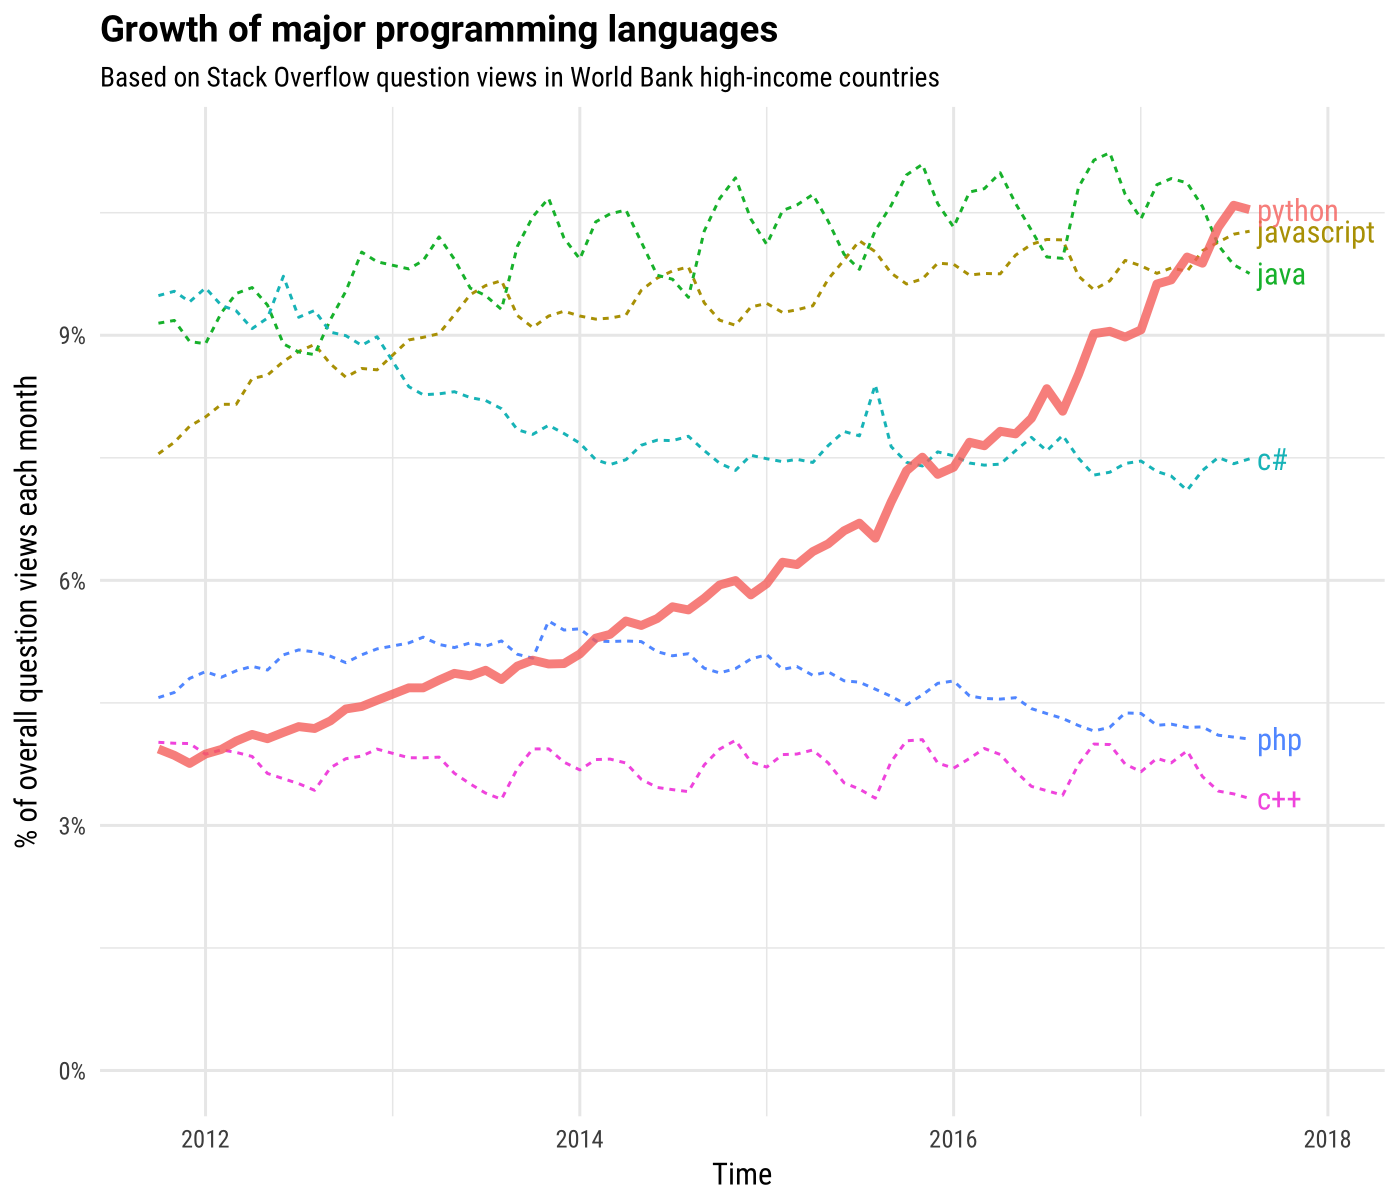
\includegraphics[width=0.95\linewidth]{assets/major_language_growth.png}
    \captionof*{figure}{ \scriptsize https://stackoverflow.blog/2017/09/06/incredible-growth-python/}
\end{frame}

\begin{frame}
    \frametitle{The Two Language Problem}
    \begin{enumerate}
        \item Languages suited for human needs, are less efficient for computers to run.
        \item Languages easy for computers to run efficiently, are correspondingly less easy for humans to use!
    \end{enumerate}
\end{frame}

\begin{frame}
    \frametitle{Why Rust?}
    Don't a lot of the `two language' problems still exist?
\end{frame}

\begin{frame}
    \frametitle{Cons of Rust}
\end{frame}


\begin{frame}
    \frametitle{State of Scientific Computing in Rust}

    Recent formation of the Rust working group within UCL's Advanced Research Computing department, to commit developer hours to open source Rust infrastructure.
\end{frame}

